\documentclass[addpoints ]{exam}

\printanswers

\CorrectChoiceEmphasis{\color{red}\bfseries}
\usepackage{amssymb, amsmath, amsfonts}
\usepackage{geometry}
\usepackage{graphicx}
\usepackage{tikz}
\usetikzlibrary{calc}
\usepackage{pgfplots}
\usepackage{multirow,array} % for payoff matrix formatting

\definecolor{crimson}{RGB}{ 170, 4, 36 }
\definecolor{darkblue}{RGB}{ 4, 47, 170 }
\definecolor{brown}{RGB}{ 111, 71, 2 }
\definecolor{periwinkle}{RGB}{ 90, 177, 204 }
\definecolor{ducksgreen}{HTML}{007030}

\geometry{left=1.0in,right=1.0in,top=1.0in,bottom=1.0in}
\pagestyle{headandfoot}
\lhead{EC327 Game Theory}
\chead{Homework 2}
\rhead{Winter 2024}
\runningheadrule

\title{
    \textbf{Econ 327: Game Theory} \\ 
    Homework $\#2$
    }
\author{University of Oregon}
\date{Due: Oct. 25$^{th}$}

% exam-type question formatting
\renewcommand{\thequestion}{\textbf{Question \arabic{question}}}
\bracketedpoints

\begin{document}

\maketitle

\begin{center}
  \gradetable[h][questions]
\end{center}

\vspace{0.5in}

\begin{center}
  \textbf{For homework assignments:}
\end{center}

\begin{itemize}

%  \item DO NOT write your name:
%  this assignment will be graded anonymously. 
%  If you want to, you can include your student ID instead.
  
  \item You will be graded on not only the content of your work
  but on how clearly you present your ideas.
  Make sure that your handwriting is legible.
  Please use extra pages if you run out of space 
  but make sure that all parts of a question 
  are in the correct order when you submit.

  \item You may choose to work with others,
  but everyone must submit to Canvas individually.

  Please include the names of everyone who you worked with 
  below your own name.
 
\end{itemize}

\vspace{1.0in}

\makebox[.6\textwidth]{Name\enspace\hrulefill}

\vspace{0.5in}

% \begin{center}
%   \fbox{\fbox{\parbox{5.5in}{\centering
%     Answer the questions in the spaces provided on the
%     question sheets. If you run out of room for an answer,
%     continue on the back of the page or another sheet of paper.}}}
% \end{center}

\newpage

\begin{questions}

%------------------------------------------------------------------%

\question
\textbf{Multiple Choice}

\begin{parts}

  \part[4]
  Consider the strategic form game below:
  \begin{table}[h!]
    \begin{center}
    \setlength{\extrarowheight}{2pt}
    \begin{tabular}{*{5}{c|}}
      \multicolumn{2}{c}{} & \multicolumn{3}{c}{$P_2$} \\\cline{3-5}
      \multicolumn{1}{c}{} &     & $x$ & $y$ & $z$ \\\cline{2-5}
      \multirow{3}*{$P_1$}  & $a$ & 1,3 & 2,2 & 3,2 \\\cline{2-5}
                           & $b$ & 2,2 & 2,2 & 4,3 \\\cline{2-5}
                           & $c$ & 1,1 & 0,2 & 1,1 \\\cline{2-5}
    \end{tabular}
    \end{center}
  \end{table}
  
  In the game above, which strategy is strictly dominated?
  
  \begin{choices}
    \choice $a$
    \choice $b$ 
    \CorrectChoice $c$
    \choice $x$
  \end{choices}

  \part[4] 
  Perform Iterative Deletion of Strictly Dominated Strategies for the same game as above all the way to completion.
  What does IDSDS tell you about the Nash equilibrium of this game?
  \begin{choices}
    \choice The NE is (a, x)
    \choice The NE is (a, y)
    \choice The NE is (Y, z)
    \CorrectChoice IESDS by itself does not reveal the NE of this game.
  \end{choices}

  \part[4]
  Consider the strategic form game below:
  \begin{table}[h!]
    \begin{center}
    \begin{tabular}{*{4}{c|}}
      \multicolumn{2}{c}{} & \multicolumn{1}{c}{$OD$} \\ \cline{3-4}
      \multicolumn{1}{c}{} &                           & $Swerve$ & $Straight$ \\ \cline{2-4}
      \multirow{2}*{$CD$}  & $Swerve$                  & -1,-1    & 1,1        \\ \cline{2-4}
                           & $Straight$                & 1,1      & -1,-1      \\ \cline{2-4}
    \end{tabular}
    \end{center}
  \end{table}

  What type of game is this?
  \begin{choices}
    \choice A zero-sum game
    \choice A coordination game 
    \CorrectChoice An anti-coordination game
    \choice A prisoners' dilemma
  \end{choices}

  \part[4]
  Consider the strategic form game below:
  \begin{table}[!h]
  \begin{center}
    \begin{tabular}{*{4}{c|}}
      \multicolumn{2}{c}{} &
      \multicolumn{1}{c}{Navratilova} \\ \cline{3-4}
      \multicolumn{1}{c}{} & & $DL$ & $CC$ \\ \cline{2-4}
      \multirow{2}*{Evert} & $DL$ & 50, 50 & 80, 20 \\ \cline{2-4}
        & $CC$ & 90,10 & 20, 80 \\ \cline{2-4} 
    \end{tabular}
  \end{center}
  \end{table}

  What is the \textit{pure strategy} Nash equilibrium?
  \begin{choices}
    \choice $(DL, DL)$
    \choice $(CC, DL)$
    \choice $(DL, CC)$
    \CorrectChoice There are no Nash equilibria in pure strategies for this game.
  \end{choices}

 \newpage
 
  \part[4]
  Cosider the same game as above.
  Suppose that Navratilova plays $DL$ with probability $p$ 
  and $CC$ with probability $(1-p)$.
  What are Evert's expected payoffs?

  \begin{choices}
    \choice $U_{Evret}(DL) = 30 - 80p$, $U_{Evret}(CC) = 70 - 20p$
    \CorrectChoice $U_{Evret}(DL) = 80 - 30p$, $U_{Evret}(CC) = 20 + 70p$
    \choice $U_{Evret}(DL) = - 60p$, $U_{Evret}(CC) = 100 + 100p$
    \choice $U_{Evret}(DL) = 90 - 40p$, $U_{Evret}(CC) = 20 + 60p$
  \end{choices}


  \part[4]
  The difference between a regular Nash equilibrium 
  and a Subgame Perfect Nash equilibrium is that:

  \begin{choices}
    \choice A Subgame Perfect Nash equilibrium assumes perfect information
    \choice Mixed strategies cannot be used in Subgame Perfect Nash equilibria
    \CorrectChoice Subgame Perfect Nash equilibria assume that players won't fall for non-credible threats
    \choice There is no difference, they are the same
  \end{choices}

  \part[4]
  Which of the following are examples of \textit{continuous} strategies?
  
  \begin{choices}
    \choice Taylor Swift's choice of which cities to go on tour in
    \CorrectChoice How much time Owen waits in line for Taylor Swift tickets
    \CorrectChoice How much money TicketMaster charges for a ticket
    \choice Jose is at home and will only go if the stadium is less than 50\% full
    \CorrectChoice Both B and C are continuous strategies
    \choice None of the above are continous strategies
  \end{choices}

  \begin{solution}
    \textbf{Note:}
    Give full credit on this question if only B is chosen or only C is chosen or both.
    I meant for the amount of time Owen waits in line to be a continuous strategy,
    but some people argued that his decision to wait or not could be discrete.
  \end{solution}

\end{parts}
  
\newpage

%------------------------------------------------------------------%

% \question
% Consider the extensive form game treee below.

% \begin{center}
%   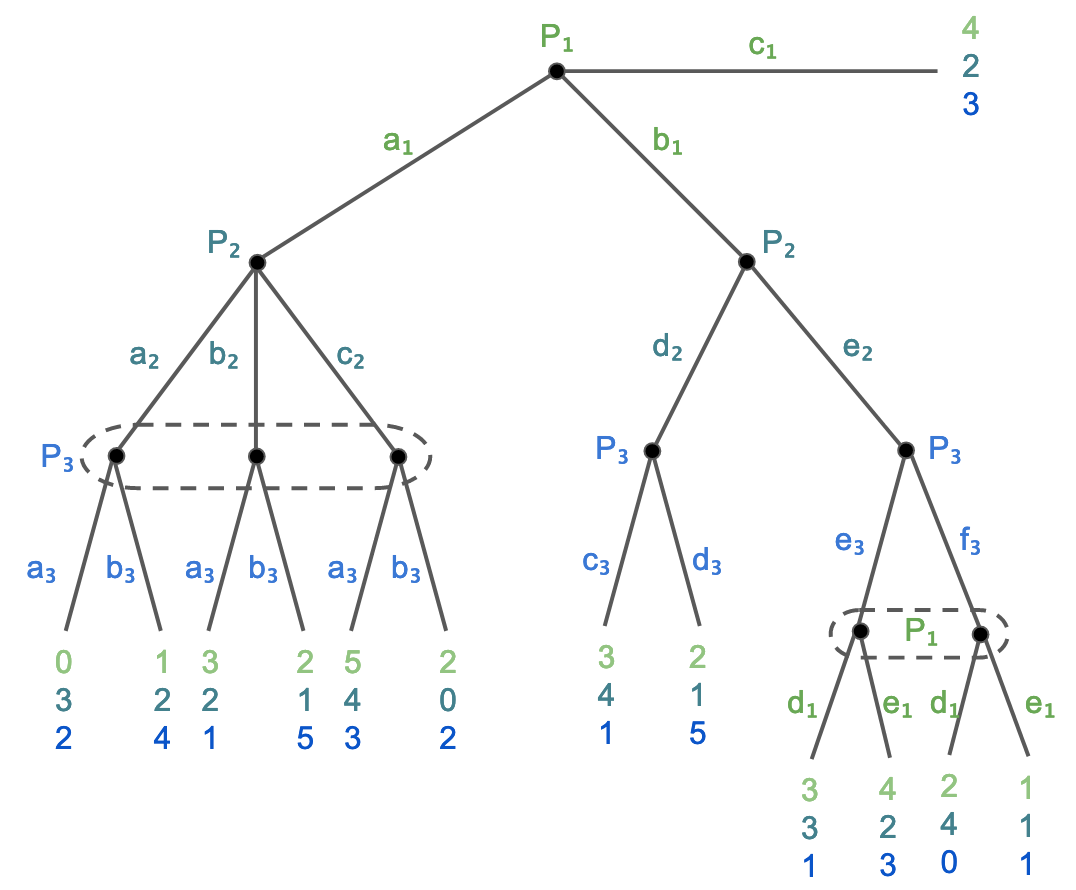
\includegraphics[width = .8\textwidth]{figures/gametree1.png}
% \end{center}

% \begin{parts}
  
%   \part[1] 
%   What should a complete strategy profile look like?

%   How many elements will each player have in their \textit{complete} strategy?

%   \part[6] Find all subgame perfect Nash equilibria in pure strategies.

%   \part[3] Can you find a Nash equilibrium that is not subgame perfect?
%   Carefully explain.

% \end{parts}

% \newpage


%------------------------------------------------------------------%

\question%[20]
Here's a little ditty, about Jack and Diane,
two American kids growing up in the heartland.
The game is below.
\footnote{Cliff Bekar, Lewis and Clark College}

  \begin{table}[h!]
    \centering
    \setlength{\extrarowheight}{2pt}
    \begin{tabular}{*{5}{c|}}
      \multicolumn{2}{c}{} & \multicolumn{3}{c}{Diane} \\\cline{3-5}
      \multicolumn{1}{c}{} &     & $x$ & $y$ & $z$ \\\cline{2-5}
      \multirow{3}*{Jack}  & $a$ & 1,1 & 2,1 & 2,0 \\\cline{2-5}
                           & $b$ & 2,3 & 0,2 & 2,1 \\\cline{2-5}
                           & $c$ & 2,1 & 1,2 & 3,0 \\\cline{2-5}
    \end{tabular}
  \end{table}

\begin{parts}
  \part[12] Find all pure Nash strategy profiles and outcomes 
    if Jack and Diane move simultaneously.
    Carefully detail and explain the strategy profiles and how they map onto your Nash outcomes.
    
    \part[16] Find all pure Nash strategy profiles and outcomes
    \textit{if Jack moves first}.
    Carefully detail and explain your strategy profiles 
    and how they map onto your Nash outcomes.
\end{parts}

\begin{solution}
  \begin{parts} 
    \part Players: $\{ \text{Jack, Diane} \}$

    Strategy sets: $S_{\text{Jack}} = \{ a, b, c \}$
    $S_{\text{Diane}} = \{ x, y, z \}$

    For Jack, $b$ and $c$ are best responses to $x$,
    $a$ is BR to $y$,  
    and $c$ is BR to $z$.

    For Diane, $x$ and $y$ are BR to $a$,
    $x$ is BR to $b$,
    and $z$ is BR to $c$.

    There are two strategy profiles where each player's best responses intersect:

    \begin{itemize}
      \item $N_1 = \left( b, x \right)$ results in payoffs (2,3)

      Jack's strategy is to choose $b$, 
      Diane's strategy is to choose $x$.
      Neither have regrets about their strategy choice;
      given that Jack is choosing $b$, Diane can't get a higher payoff by deviating.
      Given that Diane is playing $x$, Jack is indifferent between playing $b$ and $c$ but he can't get a strictly higher payoff by deviating. 
      The resulting outcome is that Jack gets $2$, 
      Diane gets $3$.

      \item $N_2 = \left( a, y \right)$ results in payoffs (2,1)

      Jack's strategy is $a$, Diane's is $y$. 
      When Jack plays $a$, Dianne is indifferent between $x$ and $y$, but
      still cannot deviate to a strictly higher payoff.
      When Diane plays $y$, Jack's best response is $a$ because $2>\{0,1\}$. 
      The outcome is that Jack gets $2$ and Diane gets $1$.

    \end{itemize}

    These are the only two \textit{pure strategy} Nash equilibria
    because there are no other intersections of pure strategy best responses.
    Note that even though $N_1$ Pareto dominates $N_2$ 
    (Jack is indifferent; $2=2$, and Diane is better off; $3>1$),
    there is no \textit{unilateral} deviation that would reach $N_1$
    from $N_2$.


    \part
    See the extensive form game tree below.

    Now the strategy sets are: 

    $S_{\text{Jack}} = \{ a, b, c \}$
    because Jack still has only one decision node.

    $S_{\text{Diane}}$ =  any combination $ \{ s_1 s_2 s_3 \}; \ \forall s \in
    \{x,y,z\}$; where $s$ can be either $x$, $y$, or $z$ at each of her
    information sets (labelled 1,2,3 on the game tree below). 

    I represented each of Diane's strategies as a triple where the first letter
    represents her choice at node 1, second letter at node 2, and third letter
    at node 3. So for example, $xyz$ would be the strategy where she chooses
    $x$ in node $1$, $y$ in node $2$, and $z$ in node $3$. 

    \begin{itemize}

      \item 
      $\mathbf{N_1} = \left( \mathbf{a}, \ \mathbf{y_1} x_2 s_3 \right)$ 
      
      where:
      \begin{itemize}
          \item $s_3$ is $\mathbf{x}$ or $\mathbf{y}$ or $\mathbf{z}$ 
      \end{itemize}

      Any set of strategies in which Jack chooses $a$
      and Diane chooses $y$ in node $1$ 
      but doesn't choose $z$ at node $3$
      would result in an equilibrium outcome of 
      $({\color{red} 2},{\color{blue} 1})$
      where Jack cannot deviate to a higher payoff than $2$,
      and Diane also has no regrets with choosing $y$.

      The payoffs obtained in this equilibrium are $({\color{red} 2}, {\color{blue} 1})$

      \item 
        $\mathbf{N_2} = \left( \mathbf{b}, \ s_1 \mathbf{x_2} s_3 \right) $
      
      where:
      \begin{itemize}
          \item $s_1$ could be $\mathbf{x}$, $\mathbf{y}$; 
          \item $s_3$ could be either $\mathbf{x}$, $\mathbf{y}$, or $\mathbf{z}$.
      \end{itemize}

      Any set of strategies in which Jack chooses $b$,
      Diane is indifferent between $x$ and $y$ at node 1 which is not on the equilibrium path of play,
      and Diane chooses $x_2$ given that jack chooses $b$. 

      The equilibrium outcome of any of these Nash strategy profiles
      would be $({\color{red} 2}, {\color{blue} 3})$

    \end{itemize}

  \end{parts}

\begin{center}
  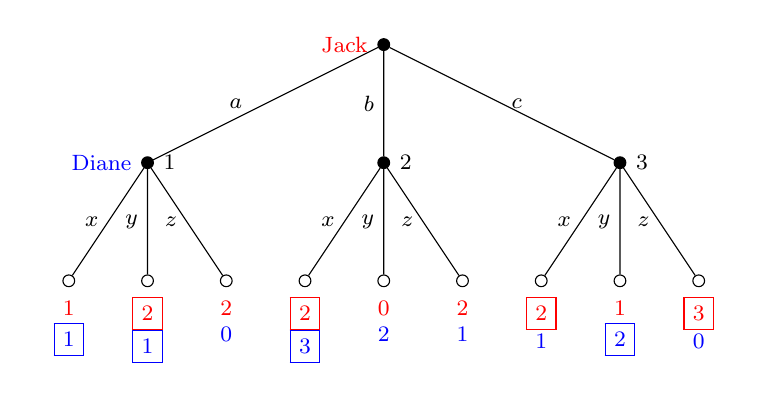
\begin{tikzpicture}[font=\footnotesize]
    \tikzstyle{solid node}=[circle,draw,inner sep=1.5,fill=black]
    \tikzstyle{hollow node}=[circle,draw,inner sep=1.5]
    \tikzstyle{level 1}=[level distance=15mm,sibling distance=3cm]
    \tikzstyle{level 2}=[level distance=15mm,sibling distance=1cm]
    \tikzstyle{level 3}=[level distance=15mm,sibling distance=.5cm]
    
    \node(0)[solid node,label=left:{\color{red} Jack}]{}
        child{node(1)[solid node,label=left:{\color{blue} Diane },label=right:{$1$}]{}
            child{node[hollow node,label=below:{
                \begin{tabular}{c}
                     {\color{red} 1}  \\
                     {\color{blue} \boxed{1}} 
                \end{tabular}
            }]{} edge from parent[] node[left]{$x$}}
            child{node[hollow node,label=below:{
                \begin{tabular}{c}
                  {\color{red} \boxed{2}}  \\
                     {\color{blue} \boxed{1}} 
                \end{tabular}
            }]{} edge from parent node[left]{$y$}}
            child{node[hollow node,label=below:{
                \begin{tabular}{c}
                     {\color{red} 2}  \\
                     {\color{blue} 0} 
                \end{tabular}
            }]{} edge from parent[ ] node[left]{$z$}}
            edge from parent node[left,xshift=-5]{$a$}
        }
        child{node(2)[solid node,label=right:{$2$}]{}
            child{node[hollow node,label=below:{
                \begin{tabular}{c}
                  {\color{red} \boxed{2}}  \\
                     {\color{blue} \boxed{3}} 
                \end{tabular}
            }]{} edge from parent[] node[left]{$x$}}
            child{node[hollow node,label=below:{
                \begin{tabular}{c}
                     {\color{red} 0}  \\
                     {\color{blue} 2} 
                \end{tabular}
            }]{} edge from parent[ ] node[left]{$y$}}
            child{node[hollow node,label=below:{
                \begin{tabular}{c}
                     {\color{red} 2}  \\
                     {\color{blue} 1} 
                \end{tabular}
            }]{} edge from parent[ ] node[left]{$z$}}
            edge from parent node[left]{$b$}
        }
        child{node(3)[solid node,label=right:{$3$}]{}
            child{node[hollow node,label=below:{
                \begin{tabular}{c}
                  {\color{red} \boxed{2}}  \\
                     {\color{blue} 1} 
                \end{tabular}
            }]{} edge from parent[ ] node[left]{$x$}}
            child{node[hollow node,label=below:{
                \begin{tabular}{c}
                     {\color{red} 1}  \\
                     {\color{blue} \boxed{2}} 
                \end{tabular}
            }]{} edge from parent[] node[left]{$y$}}
            child{node[hollow node,label=below:{
                \begin{tabular}{c}
                  {\color{red} \boxed{3}}  \\
                     {\color{blue} 0} 
                \end{tabular}
            }]{} edge from parent[ ] node[left]{$z$}}
            edge from parent node[right]{$c$}
        };
\end{tikzpicture}

\end{center}

\end{solution}

\newpage

\question

Consider the strategic form game below:

\begin{table}[!h]
  \begin{center}
    \begin{tabular}{*{6}{c|}}
      \multicolumn{2}{c}{} & \multicolumn{4}{c}{$P_2$} \\ \cline{3-6}
      \multicolumn{1}{c}{} &  & $A$ & $B$ & $C$ & $D$ \\ \cline{2-6} 
      \multirow{4}*{$P_1$}
      & $H$ & 10,  1 & -3,  1 &  0,  1 &  3,  1 \\ \cline{2-6}
      & $J$ & 16, -2 &  6,  6 &  1, -1 &  4,  0 \\ \cline{2-6} 
      & $K$ & 11,  1 &  0,  3 &  2,  2 & 10, 15 \\ \cline{2-6} 
      & $L$ & 13, 10 & -1, 16 &  4, 12 &  5, 20 \\ \cline{2-6} 
  \end{tabular}
  \end{center}
\end{table}

\begin{parts}
 
  \part[12] 
  Use Iterated Deletion of Strictly Dominated Strategies
  and write out a simplified game table with any remaining cells.

  \begin{solution}
    
    \begin{itemize}
      \item Step 1: $H$ is strictly dominated by $J$, eliminate $H$
      \item Step 2: $A$ and $C$ are strictly dominated by $B$, eliminate $A$ and $C$
      \item Step 3: $L$ is strictly dominated by $K$, eliminate $L$
    \end{itemize}

    \begin{center}
      \begin{tabular}{*{4}{c|}}
        \multicolumn{2}{c}{} & \multicolumn{2}{c}{$P_2$} \\ \cline{3-4}
        \multicolumn{1}{c}{} & & $B$ & $D$ \\ \cline{2-4}
        \multirow{2}*{$P_1$}
        & $J$ & \underline{6},\underline{6} &  4, 0 \\ \cline{2-4}
        & $K$ & 0,3 & \underline{10},\underline{15} \\ \cline{2-4}
      \end{tabular}
    \end{center}
  \end{solution}


  \part[8]
  Find all Nash equilibria in \textit{pure strategies}.

  \begin{solution}
      
    The best response to $B$ is $J$,
    and the best response to $J$ is $B$ 
    so $\mathbf{(J,B)}$ is one Nash equilibrium.

    The best response to $D$ is $K$,
    and the best response to $K$ is $D$ 
    so $\mathbf{(K,D)}$ is the other PSNE.

    \par\noindent\rule{\textwidth}{0.4pt}

    Partial credit may be awarded for an answer that is consistent with mistakes made in 
    eliminating strictly dominated strategies in part $a$.

  \end{solution}
  
  \part[6]
  Explain why you know that the strategies you found in part b are Nash equilibria.

  \begin{solution}
  
      These are they only pure strategy NE because we eliminated all strategies in part (a)
    that will never be played in any NE.
    We also found the intersection of either players best responses in the table from (a)
    which is the definition of a NE.

  \end{solution}
  
  % \part[6] 
  % Define mixed strategies for each player
  % using any pure strategies left after IDSDS.
  % Make sure to define all variables you introduce.

  % \begin{solution}
    
  %   Let $\alpha$ be the probability that $P_1$ plays $J$.

  %   Player 1's mixed strategy will be $\mathbf{(\alpha J, (1-\alpha) K)}$ 
  %   (and zero weight on $H$ and $L$).

  %   Let $\beta$ be the probability that $P_2$ plays $B$.

  %   Player 2's mixed strategy will be $\mathbf{(\beta B, (1-\beta) D)}$
  %   (and zero weight on $A$ and $C$). 

  %   \par\noindent\rule{\textwidth}{0.4pt}

  %   The notation doesn't have to match, 
  %   but a correct answer will have one probability associated with each player
  %   and the remaining probability on the proper player's other strategy played in equilibrium.

  % \end{solution}

  % \section*{Extra Credit}

  % \bonuspart[4]
  % Graph each player's expected utilities as functions of the 
  % other players' mixed strategy you defined in part (c).

  % \begin{solution}

  %   \begin{minipage}{.5\textwidth}
  %     \centering
  %      \begin{tikzpicture}
  %        \begin{axis}[
  %          width=.95\textwidth,
  %          xlabel={$\alpha$},
  %          % ylabel={Player 2's Expected Utility}
  %          xmin=0, xmax=1,
  %          ymin=0, ymax=16,
  %          ]
  %          % EU(D)
  %          \addplot [
  %            domain=0:1,
  %            samples=10,
  %            color=green,
  %          ]
  %          {15 - 15*x};
  %          \addlegendentry{\(EU_2(D)=15-15\alpha\)}
  %          % EU(B)
  %          \addplot [
  %            domain=0:1,
  %            samples=10,
  %            color=purple,
  %          ]
  %          {3 + 3*x};
  %          \addlegendentry{\(EU_2(B)=3+3\alpha\)}

  %        \end{axis} 
  %      \end{tikzpicture}
  %   \end{minipage}
  %   \begin{minipage}{.5\textwidth}
  %     \centering
  %      \begin{tikzpicture}
  %        \begin{axis}[
  %          width=.95\textwidth,
  %          xlabel={$\beta$},
  %          % ylabel={Player 2's Expected Utility}
  %          xmin=0, xmax=1,
  %          ymin=0, ymax=16,
  %          ]
  %          % EU(K)
  %          \addplot [
  %            domain=0:1,
  %            samples=10,
  %            color=yellow,
  %          ]
  %          {10 - 10*x};
  %          \addlegendentry{\(EU_1(K)=10-10\beta\)}
  %          % EU(J)
  %          \addplot [
  %            domain=0:1,
  %            samples=10,
  %            color=blue,
  %          ]
  %          {4 + 2*x};
  %          \addlegendentry{\(EU_1(J)=4+2\beta\)}

  %        \end{axis} 
  %      \end{tikzpicture}
  %   \end{minipage}

  %   When will Player 2 be indifferent between $B$ and $D$:

  %   \begin{tabular}{r c l}
  %     % $EU_2(B)$ & = & $EU_2(D)$ \\ 
  %     % $6\alpha + 3 (1-\alpha)$ & = & $0\alpha + 15(1-\alpha)$ \\
  %     % $3 + 3\alpha$ & = & $15 - 15\alpha$ \\ 
  %     $\alpha$ & = & $2/3$ \\ 
  %   \end{tabular}

  %   When will Player 1 be indifferent between $J$ and $K$:

  %   \begin{tabular}{r c l}
  %     % $EU_1(J)$ & = & $EU_1(K)$ \\ 
  %     % $6\beta + 4 (1-\beta)$ & = & $0\beta + 10(1-\beta)$ \\
  %     % $4 + 2\beta$ & = & $10 - 10\beta$ \\ 
  %     $\beta$ & = & $1/2$ \\ 
  %   \end{tabular}
  % \end{solution}


  % \bonuspart[4]
  % Solve for all Mixed Strategy Nash equilibria in this game.
  % A complete answer will include all calculations used 
  % and a graph of best response functions.

  % \begin{solution}

  %   \begin{tikzpicture}
  %     \begin{axis}[
  %       width=.8\textwidth,
  %       xlabel={$\alpha$},
  %       ylabel={$\beta$},
  %       xmin=-0.01, xmax=1.01,
  %       ymin=-0.01, ymax=1.01,
  %       xtick={0,2/3,1},
  %       ytick={0,1/2,1},
  %       ]
  %       \addplot [
  %       dashed,
  %       line width=4pt,
  %       const plot,
  %       color=purple
  %       ] coordinates {
  %       (0,0)
  %       (2/3,0)
  %       (2/3,1)
  %       (1,1)
  %       };
  %       \addlegendentry{\(BR_2(\alpha)\)}
  %       \addplot [
  %       dashed,
  %       line width=4pt,
  %       const plot,
  %       color=blue,
  %       ] coordinates {
  %       (0,0)
  %       (0,1/2)
  %       (1,1/2)
  %       (1,1)
  %       };
  %       \addlegendentry{\(BR_1(\beta)\)}
  %     \end{axis}
      
  %   \end{tikzpicture}

  %   \textbf{MSNE:} $\sigma_1 = (2/3 B, 1/3 D), \sigma_2 = (1/2 J, 1/2 K) $
  % \end{solution}

\end{parts}

\newpage

\question[10] 
The countries of Oceania and Eurasia are at war.
As depicted in the figure, Oceania has four cities —
Argula, Betra, Carnat, and Dussel — 
and it is concerned that one of them is to be bombed by Eurasia.
The bombers could come from either base Alpha,
which can reach the cities of Argula and Betra;
or from base Beta, which can reach either Carnat or Dussel.
Eurasia decides which one of these four cities to attack.
Oceania doesn’t know which one has been selected,
but does observe the base from which the bombers are flying.
After making that observation, Oceania decides which one 
(and only one) of its four cities to evacuate.

Assign a payoff of 2 to Oceania
if it succeeds in evacuating the city that is to be bombed
and a payoff of 1 otherwise.
Assign Eurasia a payoff of 1 if the city it bombs was not evacuated
and a zero payoff otherwise.
Write down the extensive form game.
\footnote{Harrington \textit{Games, Strategies, and Decision Making}}

%\vspace{-5cm}
\begin{figure}[!h]
  \centering
  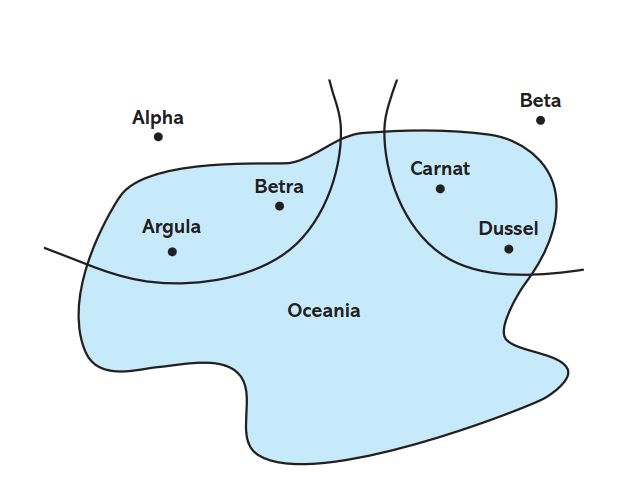
\includegraphics[width=.4\linewidth]{figures/figPR2.1.png} 
\end{figure}

\begin{solution}
  \begin{center}
    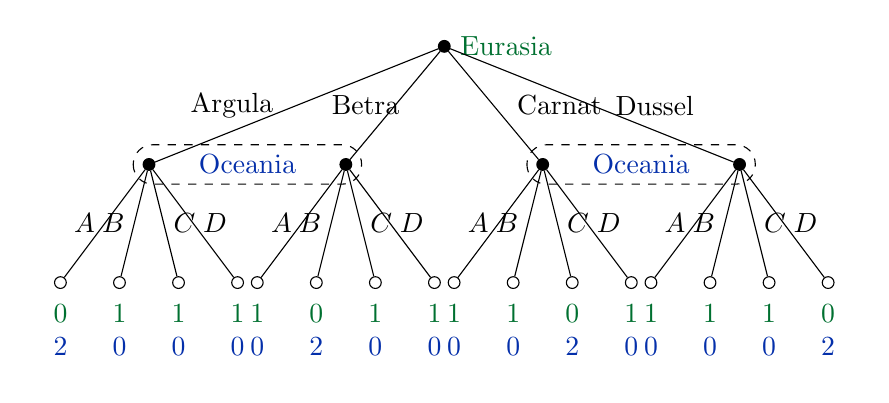
\begin{tikzpicture}[
% font=\footnotesize
]
    \tikzstyle{solid node}=[circle,draw,inner sep=1.5,fill=black]
    \tikzstyle{hollow node}=[circle,draw,inner sep=1.5]
    \tikzstyle{level 1}=[level distance=15mm,sibling distance=2.5cm]
    \tikzstyle{level 2}=[level distance=15mm,sibling distance=.75cm]
    \tikzstyle{level 3}=[level distance=15mm,sibling distance=0.5cm]
    
    \node(0)[solid node,label=right:{\color{ducksgreen} Eurasia}]{}
        child{node(1)[solid node,label=above left:{ }]{}
            child{node[hollow node,label=below:{
                \begin{tabular}{c}
                     {\color{ducksgreen} 0}  \\
                     {\color{darkblue} 2} 
                \end{tabular}
            }]{} edge from parent node[left]{$A$}}
            child{node[hollow node,label=below:{
                \begin{tabular}{c}
                     {\color{ducksgreen} 1}  \\
                     {\color{darkblue} 0} 
                \end{tabular}
            }]{} edge from parent node[left]{$B$}}
            child{node[hollow node,label=below:{
                \begin{tabular}{c}
                     {\color{ducksgreen} 1}  \\
                     {\color{darkblue} 0} 
                \end{tabular}
            }]{} edge from parent node[right]{$C$}}
            child{node[hollow node,label=below:{
                \begin{tabular}{c}
                     {\color{ducksgreen} 1}  \\
                     {\color{darkblue} 0} 
                \end{tabular}
            }]{} edge from parent node[right]{$D$}}
            edge from parent node[left,xshift=-5]{Argula}
        }
        child{node(2)[solid node,label=above right:{ }]{}
            child{node[hollow node,label=below:{
                \begin{tabular}{c}
                     {\color{ducksgreen} 1}  \\
                     {\color{darkblue} 0} 
                \end{tabular}
            }]{} edge from parent node[left]{$A$}}
            child{node[hollow node,label=below:{
                \begin{tabular}{c}
                     {\color{ducksgreen} 0}  \\
                     {\color{darkblue} 2} 
                \end{tabular}
            }]{} edge from parent node[left]{$B$}}
            child{node[hollow node,label=below:{
                \begin{tabular}{c}
                     {\color{ducksgreen} 1}  \\
                     {\color{darkblue} 0} 
                \end{tabular}
            }]{} edge from parent node[right]{$C$}}
            child{node[hollow node,label=below:{
                \begin{tabular}{c}
                     {\color{ducksgreen} 1}  \\
                     {\color{darkblue} 0} 
                \end{tabular}
            }]{} edge from parent node[right]{$D$}}
            edge from parent node[left,xshift=5]{Betra}
        }
        child{node(3)[solid node,label=above right:{ }]{}
            child{node[hollow node,label=below:{
                \begin{tabular}{c}
                     {\color{ducksgreen} 1}  \\
                     {\color{darkblue} 0} 
                \end{tabular}
            }]{} edge from parent node[left]{$A$}}
            child{node[hollow node,label=below:{
                \begin{tabular}{c}
                     {\color{ducksgreen} 1}  \\
                     {\color{darkblue} 0} 
                \end{tabular}
            }]{} edge from parent node[left]{$B$}}
            child{node[hollow node,label=below:{
                \begin{tabular}{c}
                     {\color{ducksgreen} 0}  \\
                     {\color{darkblue} 2} 
                \end{tabular}
            }]{} edge from parent node[right]{$C$}}
            child{node[hollow node,label=below:{
                \begin{tabular}{c}
                     {\color{ducksgreen} 1}  \\
                     {\color{darkblue} 0} 
                \end{tabular}
            }]{} edge from parent node[right]{$D$}}
            edge from parent node[right,xshift=5]{Carnat}
        }
        child{node(4)[solid node,label=above right:{ }]{}
            child{node[hollow node,label=below:{
                \begin{tabular}{c}
                     {\color{ducksgreen} 1}  \\
                     {\color{darkblue} 0} 
                \end{tabular}
            }]{} edge from parent node[left]{$A$}}
            child{node[hollow node,label=below:{
                \begin{tabular}{c}
                     {\color{ducksgreen} 1}  \\
                     {\color{darkblue} 0} 
                \end{tabular}
            }]{} edge from parent node[left]{$B$}}
            child{node[hollow node,label=below:{
                \begin{tabular}{c}
                     {\color{ducksgreen} 1}  \\
                     {\color{darkblue} 0} 
                \end{tabular}
            }]{} edge from parent node[right]{$C$}}
            child{node[hollow node,label=below:{
                \begin{tabular}{c}
                     {\color{ducksgreen} 0}  \\
                     {\color{darkblue} 2} 
                \end{tabular}
            }]{} edge from parent node[right]{$D$}}
            edge from parent node[right,xshift=5]{Dussel}
        };

    % information set
    \draw[dashed,rounded corners=7]($(1)+(-.2,.25)$)rectangle($(2)+(.2,-.25)$);
    \draw[dashed,rounded corners=7]($(3)+(-.2,.25)$)rectangle($(4)+(.2,-.25)$);
    % specify movers
    \node at ($.5*(1)+.5*(2)$) {\color{darkblue} Oceania};
    \node at ($.5*(3)+.5*(4)$) {\color{darkblue} Oceania};
\end{tikzpicture}
 
  \end{center} 

  Note that $A$, $B$, $C$, and $D$ in the last row are short for the city names.
  Eurasia acts first, so the initial node is labelled accordingly.
  Oceania has only two info sets which are represented with the dashed ovals.
  The $(0,2)$ or $(1,0)$ payoff sets correspond to Oceania choosing the same city that is bombed,
  or choosing a different city respectively.
\end{solution}

\newpage

\question[10] 
A game theorist is walking down the street in his neighborhood and finds \$20.
Just as he picks it up, two neighborhood kids, 
Jane and Tim,
run up to him, asking if they can have it.
Because game theorists are generous by nature, 
he says he's willing to let them have the \$20,
but only according to the following procedure:
Jane and Tim are each to submit a written request 
as to their share of the \$20. 
Let $t$ denote the amount that Tim requests for himself
and $j$ be the amount that Jane requests for herself.
Tim and Jane must choose $j$ and $t$ from the interval
$[0,20]$.
If $j + t \leq 20$, then the two receive what they requested,
and the remainder, $20 - j - t$, is split equally between them.
If, however, $j + t > 20$, then they get nothing, and the game theorist keeps the \$20.
Tim and Jane are the players in this game.
Assume that each of them has a payoff equal to the amount of money that he or she receives. 
Find all Nash equilibria.
\footnote{Harrington \textit{Games, Strategies, and Decision Making}}

%\vspace{-5cm}

\begin{solution}
  Tim's best response rule:
  $$ 
  BR_t(j) = \begin{cases}
    20 - j & \text{ if } j < 20 \\
    [0,20] & \text{ if } j = 20
    \end{cases}
  $$
  Jane's best response rule:
  $$ 
  BR_j(t) = \begin{cases}
    20 - t & \text{ if } t < 20 \\
    [0,20] & \text{ if } t = 20
    \end{cases}
  $$

  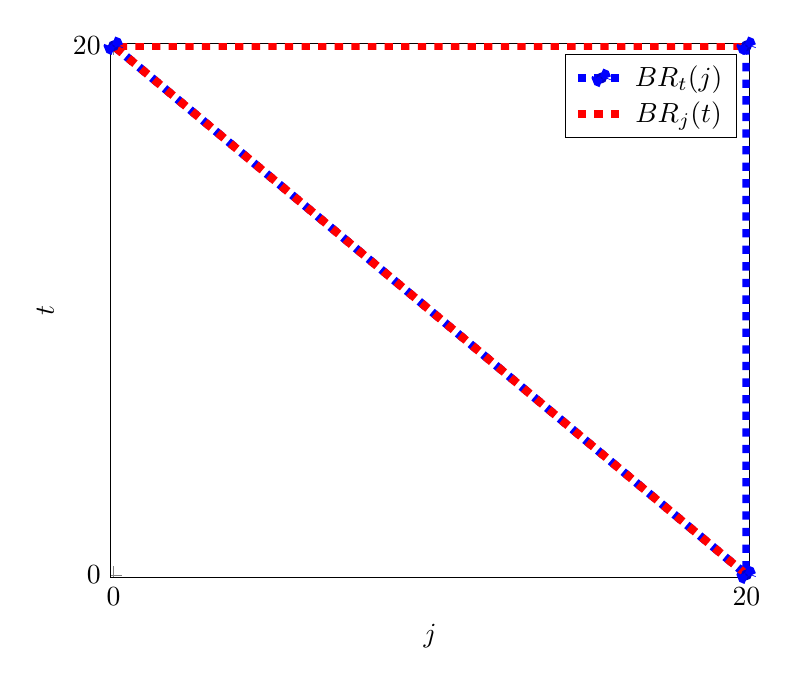
\begin{tikzpicture}
    \begin{axis}[
      width=.8\textwidth,
      xlabel={$j$},
      ylabel={$t$},
      xmin=-0.1, xmax=20.1,
      ymin=-0.1, ymax=20.1,
      xtick={0,20},
      ytick={0,20},
      ]
      \addplot+ [
      dashed,
      line width=3pt,
      color=blue,
      ] 
      coordinates
      {
      (0, 20)
      (20, 0)
      (20, 20)
      };
      \addlegendentry{\(BR_t(j)\)}
      \addplot [
      dashed,
      line width=3pt,
      color=red,
      ] 
      coordinates
      {
        (20,0)
        (0, 20)
        (20,20)
      };
      \addlegendentry{\(BR_j(t)\)}
    \end{axis}
  \end{tikzpicture}

  The NE are any points on the graph where the $BR_j(t) = t$ and $BR_t(j) = t$.
  This includes the diagonal line which is the set of all pairs,
  $j$ and $t$ such that $j + t = 20$ where $j,t<20$.
  When $j=20$, there is one NE when $t=0$ and another when $t=20$.
  When $t=20$, there is one NE when $j=0$ (and $j=20$ is still NE).

\end{solution}

\newpage

%------------------------------------------------------------------

% \question 

% Consider a situation in which a student can decide to cheat or be honest on an exam.
% If the faculty thinks the student has cheated, 
% the faculty member has to decide whether to expel them from the college
% or refer them to the Honor Board. 
% The Honor Board has to decide whether to expel the student or find them innocent.
% The payoffs are ordered, student, faculty, and college.
% Assume the board shares the college's payoffs. 
% \footnote{Cliff Bekar, Lewis and Clark College}

% \begin{figure}[!h]
%   \centering
%   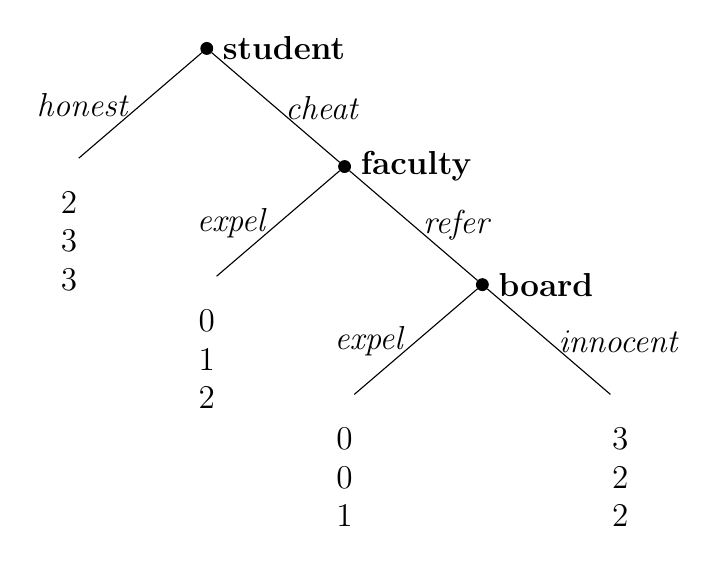
\begin{tikzpicture}[scale=1.0,font=\large]
\tikzstyle{solid node}=[circle,draw,inner sep=1.5,fill=black]
\tikzstyle{level 1}=[level distance=15mm,sibling distance=3.5cm]
\tikzstyle{level 2}=[level distance=15mm,sibling distance=3.5cm]
\tikzstyle{level 3}=[level distance=15mm,sibling distance=3.5cm]

\node(0)[solid node,label=right:{\textbf{student}}]{}
    child{node[label=below:{
            \begin{tabular}{c}
                 {2} \\
                 {3} \\
                 {3} \\
            \end{tabular}
        }]{} 
    edge from parent node[left]{\textit{honest}}}
    child{node[solid node,label=right:{\textbf{faculty}}]{} 
        child{node(1)[label=below:{
            \begin{tabular}{c}
                 {0}  \\
                 {1} \\
                 {2} \\
            \end{tabular}
        }]{} 
        edge from parent node[left]{\textit{expel}} 
        }
        child{node(2)[solid node, label=right:{\textbf{board}}]{} 
            child{node[label=below:{
                \begin{tabular}{c}
                    {0} \\
                    {0} \\
                    {1} \\
                \end{tabular}
                }]{} 
            edge from parent node[left]{\textit{expel}} 
            }
            child{node[label=below:{
                \begin{tabular}{c}
                     {3} \\
                     {2} \\
                     {2} \\
                \end{tabular}
            }]{} 
            edge from parent node[right]{\textit{innocent}} 
            }
        edge from parent node[right]{\textit{refer}} 
        }
    edge from parent node[right]{\textit{cheat}}
    };
    
\end{tikzpicture}

% \end{figure}

% \begin{parts}
%   \part[2] Find the Subgame Perfect Nash Equilibrium.

%   \part[6] Assume now that the board acts like $Nature$, making no deliberate choice 
%   but instead expels a guilty student $q\%$ of the time.
%   Find All SGPN as a function of $q$.

%   \part[2] Relative to the pure threat of explusion alone, who gains and who loses
%   from the existence of an honor board that expels probabalistically?

% \end{parts}

% \newpage

% %------------------------------------------------------------------

% \question

% The players in the following game are $Bush$ and $Saddam$. 
% $Bush$ suspects $Saddam$ of having Weapons of Mass Destruction (WMD).
% Assume for the game that $Saddam$ does have WMD. 
% $Bush$ can rely on $inspections$ or $invade$.
% $Saddam$ can $hide$ his WMD or $destroy$ them.
% \footnote{Cliff Bekar, Lewis and Clark College}

% \begin{table}[h!]
%   \begin{center}
%   \begin{tabular}{*{4}{c|}}
%     \multicolumn{2}{c}{} & \multicolumn{1}{c}{$Bush$} \\\cline{3-4}
%     \multicolumn{1}{c}{} & & $Invade$ & $Inspect$ \\\cline{2-4}
%     \multirow{2}*{$Saddam$}  & $Hide$ & -2,2 & 3,0 \\\cline{2-4}
%                          & $Destroy$ & -1,-3 & 0,1 \\\cline{2-4}
%   \end{tabular}
%   \end{center}
% \end{table}

% \begin{parts}

%   \part[4] 
%   Plot the expected values of each player's relevant strategies and find the mixed strategy Nash probabilities.

%   \part[4]
%   Plot each agent's Best Response Functions. 
%   Carefully:
  
%   \begin{subparts}
%     \subpart label your graph,
%     \subpart indicate all Nash equilibria, 
%     \subpart and explain your answer
%   \end{subparts}

%   \part[2]
%   What is the probability Bush will invade only to find no WMD?
% \end{parts}

%------------------------------------------------------------------

\end{questions}

\end{document}
